\documentclass[12pt,a4paper]{article}

\usepackage[in, plain]{fullpage}
\usepackage{array}
\usepackage{../../../pas-math}
\usepackage{../../../moncours}


%\usepackage{pas-cours}
%-------------------------------------------------------------------------------
%          -Packages nécessaires pour écrire en Français et en UTF8-
%-------------------------------------------------------------------------------
\usepackage[utf8]{inputenc}
\usepackage[frenchb]{babel}
\usepackage[T1]{fontenc}
\usepackage{lmodern}
\usepackage{textcomp}



%-------------------------------------------------------------------------------

%-------------------------------------------------------------------------------
%                          -Outils de mise en forme-
%-------------------------------------------------------------------------------
\usepackage{hyperref}
\hypersetup{pdfstartview=XYZ}
%\usepackage{enumerate}
\usepackage{graphicx}
\usepackage{multicol}
\usepackage{tabularx}
\usepackage{multirow}


\usepackage{anysize} %%pour pouvoir mettre les marges qu'on veut
%\marginsize{2.5cm}{2.5cm}{2.5cm}{2.5cm}

\usepackage{indentfirst} %%pour que les premier paragraphes soient aussi indentés
\usepackage{verbatim}
\usepackage{enumitem}
\usepackage[usenames,dvipsnames,svgnames,table]{xcolor}

\usepackage{variations}

%-------------------------------------------------------------------------------


%-------------------------------------------------------------------------------
%                  -Nécessaires pour écrire des mathématiques-
%-------------------------------------------------------------------------------
\usepackage{amsfonts}
\usepackage{amssymb}
\usepackage{amsmath}
\usepackage{amsthm}
\usepackage{tikz}
\usepackage{xlop}
%-------------------------------------------------------------------------------



%-------------------------------------------------------------------------------


%-------------------------------------------------------------------------------
%                    - Mise en forme avancée
%-------------------------------------------------------------------------------

\usepackage{ifthen}
\usepackage{ifmtarg}


\newcommand{\ifTrue}[2]{\ifthenelse{\equal{#1}{true}}{#2}{$\qquad \qquad$}}

%-------------------------------------------------------------------------------

%-------------------------------------------------------------------------------
%                     -Mise en forme d'exercices-
%-------------------------------------------------------------------------------
%\newtheoremstyle{exostyle}
%{\topsep}% espace avant
%{\topsep}% espace apres
%{}% Police utilisee par le style de thm
%{}% Indentation (vide = aucune, \parindent = indentation paragraphe)
%{\bfseries}% Police du titre de thm
%{.}% Signe de ponctuation apres le titre du thm
%{ }% Espace apres le titre du thm (\newline = linebreak)
%{\thmname{#1}\thmnumber{ #2}\thmnote{. \normalfont{\textit{#3}}}}% composants du titre du thm : \thmname = nom du thm, \thmnumber = numéro du thm, \thmnote = sous-titre du thm

%\theoremstyle{exostyle}
%\newtheorem{exercice}{Exercice}
%
%\newenvironment{questions}{
%\begin{enumerate}[\hspace{12pt}\bfseries\itshape a.]}{\end{enumerate}
%} %mettre un 1 à la place du a si on veut des numéros au lieu de lettres pour les questions 
%-------------------------------------------------------------------------------

%-------------------------------------------------------------------------------
%                    - Mise en forme de tableaux -
%-------------------------------------------------------------------------------

\renewcommand{\arraystretch}{1.7}

\setlength{\tabcolsep}{1.2cm}

%-------------------------------------------------------------------------------



%-------------------------------------------------------------------------------
%                    - Racourcis d'écriture -
%-------------------------------------------------------------------------------

% Angles orientés (couples de vecteurs)
\newcommand{\aopp}[2]{(\vec{#1}, \vec{#2})} %Les deuc vecteurs sont positifs
\newcommand{\aopn}[2]{(\vec{#1}, -\vec{#2})} %Le second vecteur est négatif
\newcommand{\aonp}[2]{(-\vec{#1}, \vec{#2})} %Le premier vecteur est négatif
\newcommand{\aonn}[2]{(-\vec{#1}, -\vec{#2})} %Les deux vecteurs sont négatifs

%Ensembles mathématiques
\newcommand{\naturels}{\mathbb{N}} %Nombres naturels
\newcommand{\relatifs}{\mathbb{Z}} %Nombres relatifs
\newcommand{\rationnels}{\mathbb{Q}} %Nombres rationnels
\newcommand{\reels}{\mathbb{R}} %Nombres réels
\newcommand{\complexes}{\mathbb{C}} %Nombres complexes


%Intégration des parenthèses aux cosinus
\newcommand{\cosP}[1]{\cos\left(#1\right)}
\newcommand{\sinP}[1]{\sin\left(#1\right)}


%Probas stats
\newcommand{\stat}{statistique}
\newcommand{\stats}{statistiques}
%-------------------------------------------------------------------------------

%-------------------------------------------------------------------------------
%                    - Mise en page -
%-------------------------------------------------------------------------------

\newcommand{\twoCol}[1]{\begin{multicols}{2}#1\end{multicols}}


\setenumerate[1]{font=\bfseries,label=\textit{\alph*})}
\setenumerate[2]{font=\bfseries,label=\arabic*)}


%-------------------------------------------------------------------------------
%                    - Elements cours -
%-------------------------------------------------------------------------------





%\makeatletter
%\renewcommand*{\@seccntformat}[1]{\csname the#1\endcsname\hspace{0.1cm}}
%\makeatother


%\author{Olivier FINOT}
\date{}
\title{}

\graphicspath{{./img/}}

\lhead{Seq 3: Fractions}
\rhead{O. FINOT}
%
%\rfoot{Page \thepage}
\begin{document}
%\maketitle




\chap[num=11, color=red]{Statistiques et probabilités}{}

\begin{myobj}
	\begin{itemize}
		
		\item Construire le symétrique d’un point ou d'une figure par rapport à une droite à la main où à l’aide d’un logiciel;
		\item Construire le symétrique d’un point ou d'une figure par rapport à un point, à la main où à l’aide d’un logiciel;
		\item Utiliser les propriétés de la symétrie axiale ou centrale;
		\item Identifier des symétries dans des figures.		
	\end{itemize}
\end{myobj}

\begin{mycomp}
	\begin{itemize}
		\item \kw{Chercher (Ch2)} :  s’engager    dans    une    démarche    scientifique, observer, questionner, manipuler, expérimenter (sur une feuille de papier, avec des objets, à l’aide de logiciels), émettre des hypothèses, chercher des exemples ou des contre-exemples, simplifier ou particulariser une situation, émettre une conjecture ;
		\item \kw{Raisonner (Ra3)} :  démontrer : utiliser un raisonnement logique et des règles établies (propriétés, théorèmes, formules) pour parvenir à une conclusion ;
		\item \kw{Communiquer (Co2)} :  expliquer à l’oral ou à l’écrit (sa démarche, son raisonnement, un calcul, un protocole   de   construction   géométrique, un algorithme), comprendre les explications d’un autre et argumenter dans l’échange ; 
		
	\end{itemize}
\end{mycomp}





\section{Effectif et fréquence}




%\begin{mydef}
%	En statistiques, in observe une \kw{population}. Sur cette population, on étudie un \kw{caractère} qui peut prendre plusieurs \kw{valeurs}.
%\end{mydef}


\begin{myex}
	On a pesé 12 téléphones portables et obtenu les poids suivants (en g) :
	
	\begin{center}
		95 ; 105 ; 100 ; 90 ; 95 ; 105 ; 95 ; 105 ; 100 ; 95 ; 100 ; 100
	\end{center}
	
	
	
	Ces données, c’est-à-dire les douze masses, constituent une série statistique.
	\begin{itemize}
		\item La \kw{population} est l'ensemble des téléphones portables.
		\item Le \kw{caractère} étudié est la masse des téléphones portables.
		\item Les \kw{valeurs} du caractère sont les quatre masses différentes obtenues : 90 95 100 105.
		%\item 	Les \kw{valeurs extrêmes} sont la plus petite et la plus grande des masses relevées : 90 et 105.
		\item L’\kw{effectif} d'une valeur du caractère est le nombre de téléphones portables dont la masse est égale à cette valeur. Par exemple, l'effectif de la valeur 95 est 4.	
		\item 	L’\kw{effectif total} de la série est le nombre total de masses relevées : 12.
		
		\item La \kw{fréquence} d'une valeur est le quotient de son effectif par l'effectif total. Par exemple la fréquence de la valeur 105 est La fréquence peut être écrite en pourcentage, en écriture décimale ou en fraction.
		%\item L’\kw{étendue} est la différence entre la valeur la plus haute et la plus basse : 105-90 = 15.
	\end{itemize}
	
	
	On résume ces informations dans un tableau :
	
	\vspace*{0.5cm}
	\begin{center}
		
	
		\begin{tabular}{|@{\ }l@{\ }|@{\ }c@{\ }|@{\ }c@{\ }|@{\ }c@{\ }|@{\ }c@{\ }|@{\ }c@{\ }|}
			\hline
			Valeur               & 90             & 95                             & 100                            & 105                            & Total             \\ \hline
			Effectif             & 1              & 4                              & 4                              & 3                              & 12                \\ \hline
			Fréquence & $\frac{1}{12}$ & $\frac{4}{12}$ = $\frac{1}{3}$ & $\frac{4}{12}$ = $\frac{1}{3}$ & $\frac{3}{12}$ = $\frac{1}{4}$ & $\frac{12}{12}=1$ \\ \hline
		\end{tabular}
	\end{center}
	
\end{myex}

\section{Représentation graphique}



\begin{myex}
	
	Les élèves d'une classe de cinquième font une étude statistique sur le nombre de sports qu’ils pratiquent.
	
	À la question «  Combien de sports pratiques-tu ? », voici les réponses des élèves :
	
	\begin{center}
		0;3;2;0;0;1;1;2;1;1;3;0;1;2;1;3;0;2;1;1;2;0;1;0;1.
	\end{center}

	On peut utiliser un diagramme en bâtons ou un diagramme circulaire pour visualiser cette série statistique.
	On a repris les données dans un tableau d’effectifs auquel on a ajouté les fréquences et les caractéristiques du diagramme circulaire :


	\begin{tabular}{|@{\ }l@{\ }|@{\ }c@{\ }|@{\ }c@{\ }|@{\ }c@{\ }|@{\ }c@{\ }|@{\ }c@{\ }|}
		\hline
		Nombre de sports pratiqués    & 0                                                   & 1                      & 2                     & 3                     & Total      \\ \hline
		Effectif                      & 7                                                   & 10                     & 5                     & 3                     & 25         \\ \hline
		Fréquence en pourcentage      & $\frac{7}{25}=28 \% $                               & $\frac{10}{25}=40 \% $ & $\frac{5}{25}=20 \% $ & $\frac{3}{25}=12 \% $ & 100 \%     \\ \hline
		Fréquence en nombre décimal   & \num{0.28}                                          & \num{0.4}              & \num{0.2}             & \num{0.12}            & 1          \\ \hline
		Angle du diagramme circ.      & $\num{0.28} \times 360\degree = \num{100.8}\degree$ & 144\degree             & 72\degree             & \num{43.2}\degree     & 360\degree \\ \hline
		%Longueur du diagramme à bande & $\num{0.28}\times 10 cm = \num{2.8}cm$              & 4 cm                   & 2 cm                  & \num{1.2}cm           & 10 cm      \\ \hline
	\end{tabular}
	
	\vspace*{0.5cm}
	
	\begin{multicols}{2}
		\begin{center}
			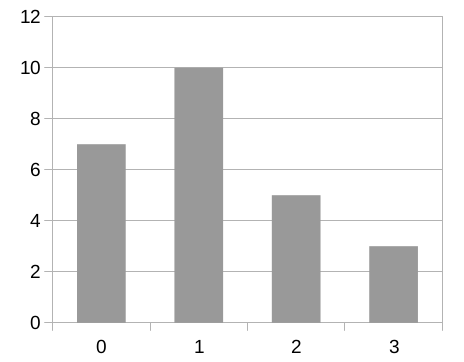
\includegraphics[scale=0.4]{baton}
		\end{center}
	
		\begin{center}
			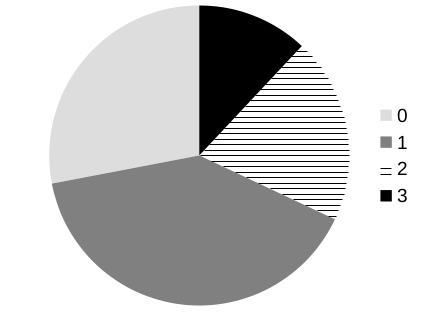
\includegraphics[scale=0.4]{circ}
		\end{center}
	\end{multicols}
	
\end{myex}

\newpage

\section{Moyenne}


\begin{mydef}
	La \kw{moyenne} d'une série statistique est le quotient de la somme des valeurs par l'effectif total (le nombre de valeurs).
\end{mydef}

\begin{myex}
	Louise a parcouru 14 km lundi, 17 km mardi, 13 km mercredi, 15 km jeudi et 11 km vendredi.
	
	\begin{equation}
		(14 + 17 + 13 + 15 + 11) \div 5  = 70 \div 5 = 14
	\end{equation}
	
	En moyenne, elle a parcouru 14 km par jour.
\end{myex}

\begin{myex}
	Un examen professionnel comporte une épreuve théorique de coefficient 3 et une épreuve pratique de coefficient 5.
	
	Un candidat a obtenu 8 à la première et 12 à la seconde. Sa moyenne $m$ est :
	
	\begin{equation*}
		m = \dfrac{8 \times 3 + 12 \times 5}{3+5}=\dfrac{84}{8} = \num{10.5}
	\end{equation*}
	
	Cette moyenne est appelée \kw{moyenne pondérée} car toute les notes n'ont pas le même <<poids>>.\\
	
	
	$\underline{Remarque}$ : Tout se passe comme si le candidat avait obtenu trois fois la note 8 et cinq fois la note 12.
	
	
\end{myex}

\section{Probabilités}

\subsection{Expérience aléatoire}

\begin{myex}
	Quand on lance une pièce de monnaie :
	\begin{itemize}
		\item On connait tous les résultats possibles (<<Pile>> ou <<Face>>).
		\item On ne peut pas prévoir le résultat qu'on va obtenir.
		\item On peut refaire l'expérience plusieurs fois.
	\end{itemize}

	C'est une \kw{expérience aléatoire}. Les résultats possibles de l'expérience sont les \kw{issues}. Ici il y a deux issues <<Pile>> et <<Face>>
\end{myex}

\subsection{\'Evénement}

\begin{mydef}
	A partir d'une expérience aléatoire on peut définir ce qu'on appelle des \kw{événements} qui sont des ensembles de résultats.
\end{mydef}

\begin{myex}
	A partir de l'expérience <<Lancer un dé à 6 faces>> on peut définir entre autres les événements suivants :
	\begin{itemize}
		\item obtenir un nombre pair (2, 4 ou 6);
		\item obtenir un 1;
		\item obtenir un résultat  inférieur ou égal à 4.
		
	\end{itemize}
\end{myex}

\subsection{Calculer une probabilité}

	\begin{mydef}
		Calculer la \kw{probabilité} d'un événement c'est estimer le <<nombre de chances>> qu'il a de se produire. C'est un nombre compris entre 0 et 1. 
		\begin{itemize}
			\item Plus un événement a de chance de se produire et plus sa probabilité va être proche de 1.
			\item Moins il a de chances de se produire et plus sa probabilité sera proche de 0.
		\end{itemize}
	
		\begin{center}
			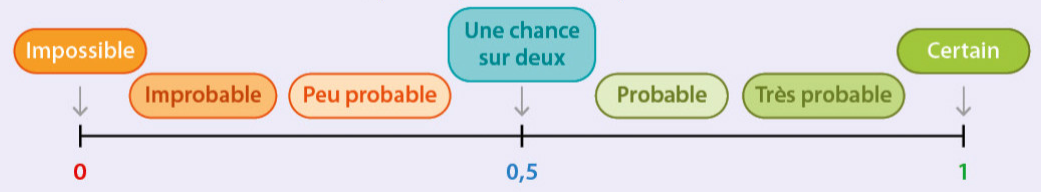
\includegraphics[scale=0.5]{proba}
		\end{center}
	
		Il y a \kw{équiprobabilité} lorsque toutes les issues d'une expérience aléatoire ont le même nombre de chance de se produire.
	\end{mydef}

	\begin{myex}
		Si on lance un dé à 6 faces, la probabilité d'obtenir
		\begin{itemize}
			\item un 1 est $\dfrac{1}{6}$;
			\item un nombre pair est $\dfrac{3}{6} = \dfrac{1}{2}$;
			\item un nombre inférieur ou égal à 4 est $\dfrac{4}{6}=\dfrac{2}{3}$.
		\end{itemize}
	\end{myex}

%	\begin{myrem}
%		La somme des probabilités de toutes les issues d'une expérience aléatoire est égale à 1.
%	\end{myrem}
	
\end{document}

